\documentclass[12pt, letterpaper]{article}
\usepackage[utf8]{inputenc}
\usepackage[english]{babel} % To obtain English text with the blindtext package
\usepackage{blindtext}
\usepackage{amsmath}
\usepackage{amssymb}
\usepackage{enumitem}
\usepackage{courier}
\usepackage{listings}
\usepackage{graphicx}
\usepackage{pgfplots}
\graphicspath{ {./images/} }

\lstdefinestyle{mystyle}{
    basicstyle=\fontsize{6}{8}\selectfont\ttfamily,
    breakatwhitespace=false,         
    breaklines=true,                 
    captionpos=b,                    
    keepspaces=true,                 
    numbers=left,                    
    numbersep=5pt,                  
    showspaces=false,                
    showstringspaces=false,
    showtabs=false,                  
    tabsize=2
}

\lstset{style=mystyle}

\title{CSCI2291 Homework 4}
\author{Jack Moffatt}
\date{February 22, 2022}


\begin{document}
\maketitle
\noindent\makebox[\linewidth]{\rule{18cm}{0.4pt}}

\section*{Problem 1}
We will use the following code as our solution:
\begin{lstlisting}[language=python]
    import pandas as pd
    import numpy as np
    from matplotlib import pyplot as plt
    
    covid_data = pd.read_csv("HW4/python/dataset/owid-covid-data.csv")
    country_labels = np.unique(covid_data.iso_code)
    country_data = np.zeros(shape=(len(country_labels),2))
    
    for i in range(0, len(country_labels)):
        code = country_labels[i]
        vax_dataset = covid_data.people_fully_vaccinated_per_hundred.loc[covid_data.iso_code == code]
        deaths_dataset = covid_data.total_deaths_per_million.loc[covid_data.iso_code == code]
        country_data[i] = [vax_dataset.max(), deaths_dataset.max()]
    
    country_data = country_data[np.logical_not(np.isnan(country_data[:,0]))]
    country_data = country_data[np.logical_not(np.isnan(country_data[:,1]))]
    
    print(f"{'Correlation Coefficent:' :<25}{round(np.corrcoef(country_data, rowvar=False)[0][1], 3)}")
    
    plt.scatter(country_data[:,0], country_data[:,1])
    plt.title("Vaccination Rate vs. Total Deaths per Million (by country)")
    plt.xlabel("Total Percentage of People Fully Vaccinated")
    plt.ylabel("Total Number of Deaths per Million People")
    plt.xlim([0,100])
    plt.ylim(bottom=0)
    plt.show()
\end{lstlisting}
There is a lot to unpack here. First, as always, we import the standard NumPy, Pandas, and Matplotlib libraries. 
Then, we load our covid data into a DataFrame, and we extract the column of country iso codes, into a list, saving 
only one copy of each code by using \texttt{np.unique}. Next, we initialize a NumPy array of zeros, with the shape of 
2 columns and 1 row for every conutry in the list of country labels.  \\ \\
Then we can loop through the list of country labels and extract the data from the vaccination percentage 
column and the total deaths per million column, and add the maximum data points from each of these series to a row in our NumPy array. Then, we clean 
our data by first removing every row with a \texttt{np.nan} value in the vaccination column and a \texttt{np.nan} 
value in the deaths column. \\ \\
Then we calculate the correlation coefficent and index into the first row and second column to get the 
corelation coefficent between the two data sets. We are given the result:
\begin{lstlisting}[language=python]
    >>> Correlation Coefficent:  0.331
\end{lstlisting}
Next, we can create a scatter plot with the vaccination percentage as our x-axis and our total deaths per million as 
our y-axis. Applying a title, labels, and scaling appropriately, we are given the graph 
\[
    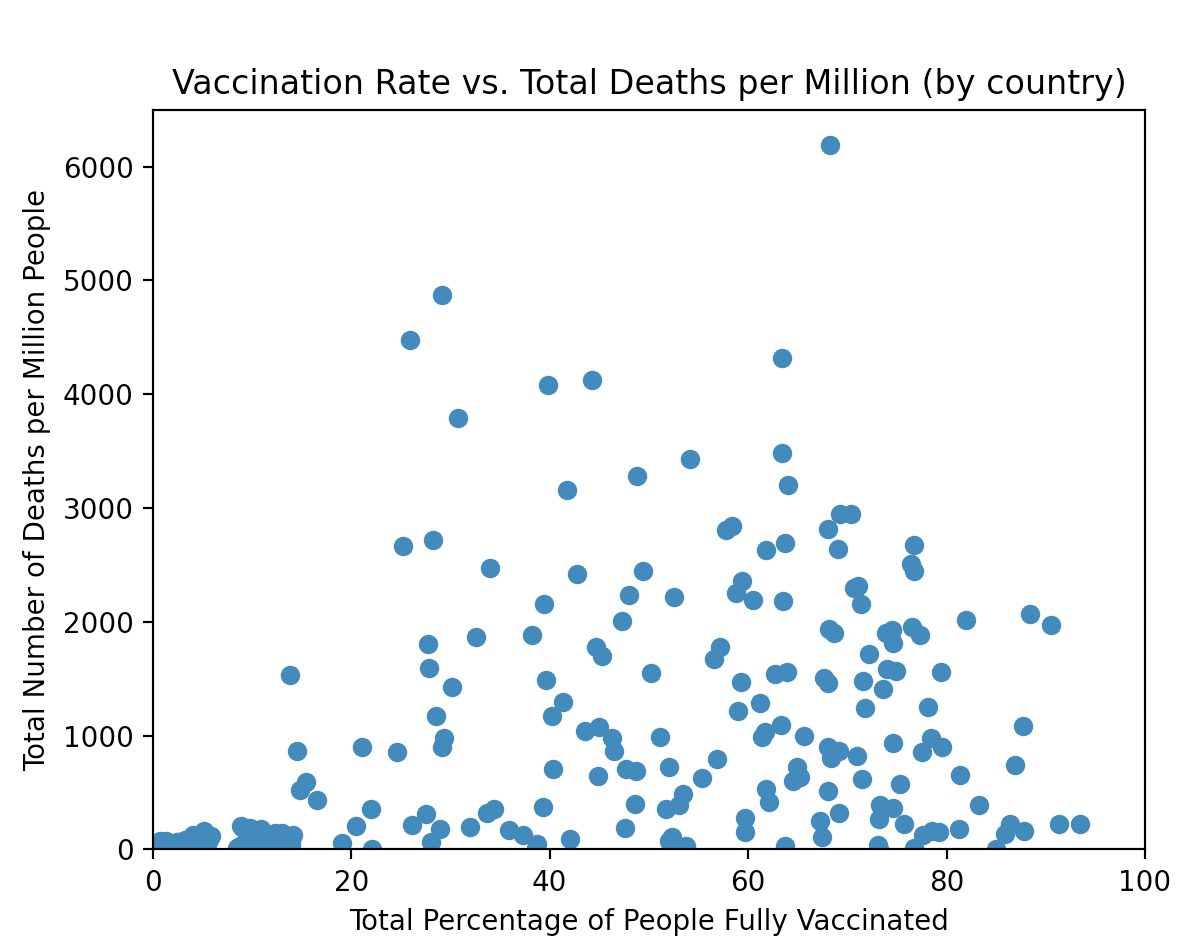
\includegraphics[scale = .33]{scatter_1.png}
\]  
Given the correlation coefficient is only $.331$, we see that there is not a very strong connection 
between our two data points. Furthermore, we can visually see that there doesn't seem to be much of a trend 
in the scatter plot. Additionally, as the correlation coefficient is positive in the relationship 
of percentage of fully vaccinated people to total deaths per million, it suggests that as vaccination 
percentage increases, there is an increase in the percentage of deaths per million.\\ \\
From the data, we can conclude that vaccination rate does not help mitigate the death rate 
due to COVID-19. 


\newpage
\noindent\makebox[\linewidth]{\rule{18cm}{0.4pt}}
\section*{Problem 2}
We will use the following code as a solution
\begin{lstlisting}[language=python]
    import pandas as pd
    import numpy as np
    from matplotlib import pyplot as plt

    covid_data = pd.read_csv("HW4/python/dataset/owid-covid-data.csv")
    country_labels = np.unique(covid_data.iso_code)
    correlations_array = np.zeros(len(country_labels))

    for i in range(0, len(country_labels)):
        code = country_labels[i]
        vax_dataset = covid_data.people_fully_vaccinated_per_hundred.loc[covid_data.iso_code == code]
        deaths_dataset = covid_data.new_deaths_smoothed_per_million.loc[covid_data.iso_code == code]
        country_data = pd.DataFrame({"people_fully_vaccinated_per_hundred" : vax_dataset, "new_deaths_smoothed_per_million" : deaths_dataset})
        country_data = country_data.loc[np.logical_not(np.isnan(vax_dataset))]
        country_data = country_data.loc[np.logical_not(np.isnan(deaths_dataset))]
        coerr_coef = country_data['people_fully_vaccinated_per_hundred'].corr(country_data['new_deaths_smoothed_per_million'])
        correlations_array[i] = coerr_coef

    correlations_array = correlations_array[np.logical_not(np.isnan(correlations_array))]
    print(f"{'Correlation Coefficent:' :<25}{round(np.median(correlations_array), 3)})

    plt.boxplot(correlations_array, notch = True)
    plt.title("Correlation Coefficents Between Vaccination Rate and \nDeath Rate per Million")
    plt.ylim([-1, 1])
    plt.show()
\end{lstlisting}
Again, we begin by importing and loading the data into a DataFrame. Again, we create a list 
of our country iso codes, and this time, we initialize a 1D NumPy array with length equal to the length 
of the country labels list. \\ \\
Again, we iterate over the list of country labels, and for each iso code in the list, we separate out 
the percentage of vaccination and the total deaths per million, this time using the smoothed version of that 
data. Each of these are pandas series, so we will create a DataFrame from these series. \\ \\
Then, using boolean indexing, we can clean the data of \texttt{np.nan} values. 
Then, we can use the pandas library to get the correlation coefficent between these two columns, 
and add the corelation coefficient to our 1D NumPy array. At the end of the for loop, we have a 1D NumPy array 
where each row corresponds to the corelation coefficient between vaccination rate and death rate per million for a specific country.
Again, we can clean our data of any \texttt{np.nan} values that may still be present. \\ \\
We see that the median of this correlation array is 
\begin{lstlisting}[language=python]
    >>>Correlation Coefficient: -0.211
\end{lstlisting} 
And, after labeling our notched box plot, we are given the visualization:
\[
    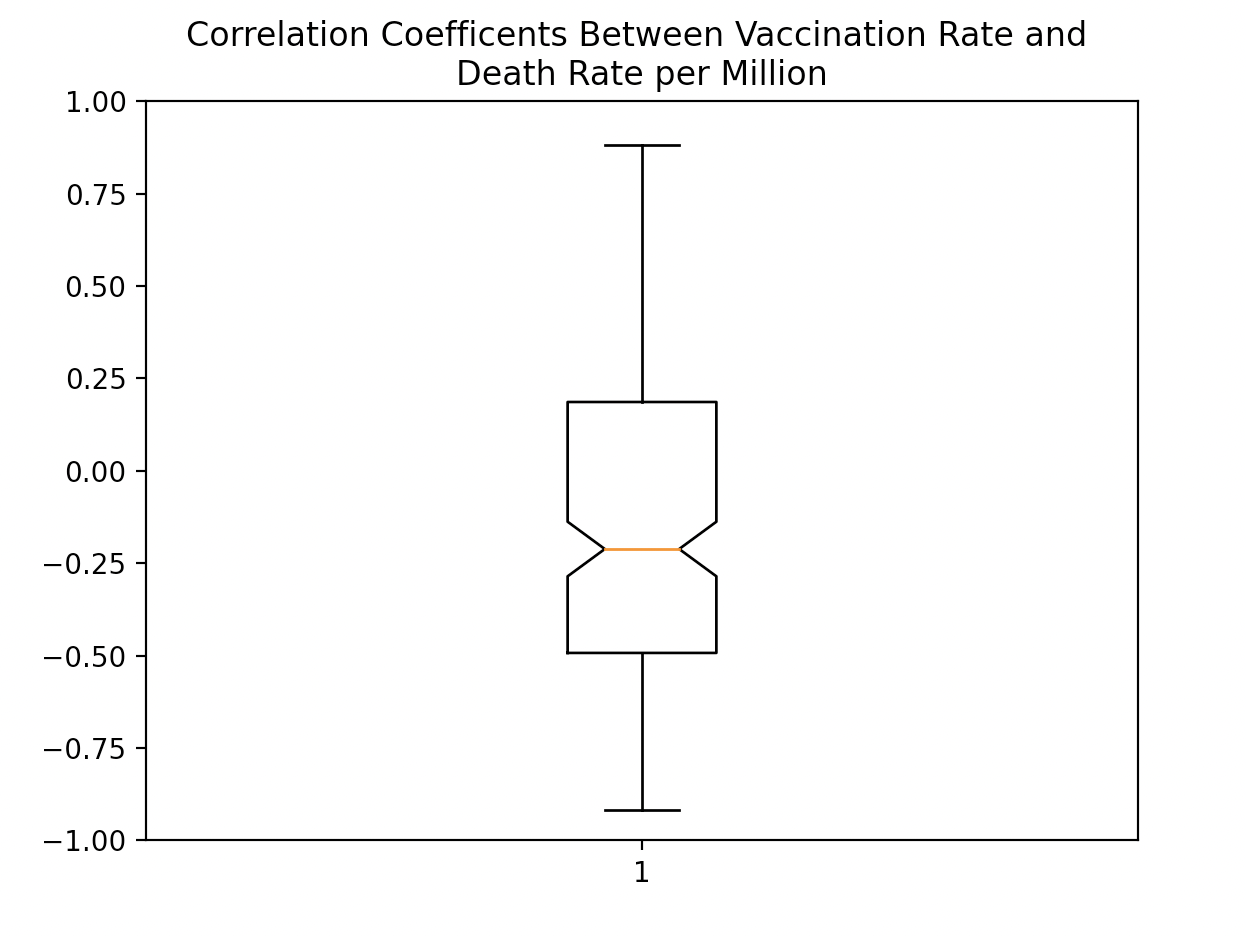
\includegraphics[scale = .33]{boxplot_2.png}
\]  
We see that the inter-quartile range of this data lies between -.5 and .25 approximately.
This suggests, that for the most part there is little corelation between vaccination rate 
and death rate. One signifigant difference between this result and the result in Problem {\bf 1}, is that now 
the correlation coefficent is negative. This means that our results suggest under this model that 
an increase in vaccination rate has an effect on decreasing the death rate. However, the magnitude of this 
correlation is still small (.221) so the data suggests there is still only a small effect. 


\newpage
\noindent\makebox[\linewidth]{\rule{18cm}{0.4pt}}
\section*{Problem 3}
\begin{enumerate}
    \item [(a)] We will use the following code as a solution:
\begin{lstlisting}[language=python]
    def iso_code_to_int(code):
        out = 0
        for i, c in enumerate(code):
            num = ord(c)
            power = len(code) - (i + 1)
            out += num * (256 ** (power))
        return out
\end{lstlisting}
    This function takes in a string, \texttt{code}. It then initializes an integer \texttt{out}, to 0. 
    Then, using Python's enumerate, it iterates over each character in the string, taking the ASCI code 
    of that character with Python's, \texttt{ord()} function. \\ \\
    Then based on the example given in the notes, it first computes the power of 256 
    given the index of the character in the string. Then, it increments \texttt{out} by the ASCI value 
    multiplied by 256 raised to the power calculated in the line above. Upon, completing the for loop, 
    the function returns \texttt{out}.
    \newpage
    \item [(b)] We will use the following code as a solution:
\begin{lstlisting}[language=python]
    import pandas as pd
    import numpy as np

    covid_data = pd.read_csv("HW4/python/dataset/owid-covid-data.csv")
    country_labels = np.unique(covid_data.iso_code)
    deaths_dict, hash_table = {}, {}

    for code in country_labels:
        max_num_deaths = covid_data.total_deaths_per_million.loc[covid_data.iso_code == code].max()
        hash_table[iso_code_to_int(code)] = code
        deaths_dict[iso_code_to_int(code)] = max_num_deaths

    deaths_data = np.array(list(deaths_dict.items()))

    first_q = np.nanquantile(deaths_data[:,1], .25)
    third_q = np.nanquantile(deaths_data[:,1], .75)

    q1, q3 = [], []

    for key in deaths_dict:
        if deaths_dict[key] <= first_q:
            q1.append(hash_table[key])
        if deaths_dict[key] >= third_q:
            q3.append(hash_table[key])

    print(f"q1: {q1}")
    print(f"q3: {q3}")
\end{lstlisting}
We begin again by importing necessary libraries, loading the data into a DataFrame, and creating a list of iso codes. 
We also initialize empty dictionaries, one for the data of deaths per country and a hash table to allow us to retrieve 
a country's iso code given its integer key. \\ \\
Then we will iterate over the list of country labels. For each iteration, we take the maximum number 
of deaths per million of the given country, then we add key-value pairs to both our hash table and our 
deaths data dictionary. \\ \\
After our for loop completes, we use the deaths deictionary to create a two dimensional NumPy array, 
where the first column is our integer iso codes, and the second column is our maximum number of deaths 
for the given country. Then, using \texttt{np.nanquantile} we take the first and third quartile points of 
our maximum number of deaths column, ignoring \texttt{np.nan} values. \\ \\
Then, we initialize two empty lists, one to hold the list of countries in the first quartile, 
and one for the countries in the third quartile. We then loop over the keys in the deaths dictionary and if the 
number of deaths for the given code is less than the first quartile value, we add the country iso code to \texttt{q1}
by retrieving the iso code from the hash table. Likewise, if the number of deaths for the country code is greater than 
the third quartile value, we add the iso code to \texttt{q3}. \\ \\
Finally, we print our two lists 
\begin{lstlisting} [language=python]
    >>>  q1: ['AGO', 'BDI', 'BEN', 'BFA', 'BTN', 'CAF', 'CHN', 'CIV', 'CMR', 'COD', 'COG', 'ERI', 'ETH', 'GAB', 'GHA', 'GIN', 'GNB', 'GNQ', 'GRL', 'HKG', 'HTI', 'ISL', 'KEN', 'KOR', 'LAO', 'LBR', 'MDG', 'MLI', 'MOZ', 'MWI', 'NER', 'NGA', 'NIC', 'NZL', 'OWID_LIC', 'PAK', 'PNG', 'RWA', 'SDN', 'SEN', 'SLB', 'SLE', 'SOM', 'SSD', 'TCD', 'TGO', 'TJK', 'TLS', 'TWN', 'TZA', 'UGA', 'UZB', 'VUT', 'YEM']
    >>>  q3: ['ABW', 'AND', 'ARG', 'ARM', 'BEL', 'BGR', 'BHS', 'BIH', 'BMU', 'BOL', 'BRA', 'CHL', 'COL', 'CZE', 'ECU', 'ESP', 'FRA', 'GBR', 'GEO', 'GIB', 'GRC', 'GRD', 'HRV', 'HUN', 'ITA', 'LCA', 'LIE', 'LTU', 'LVA', 'MDA', 'MEX', 'MKD', 'MNE', 'OWID_EUN', 'OWID_EUR', 'OWID_NAM', 'OWID_SAM', 'PER', 'POL', 'PRT', 'PRY', 'PYF', 'ROU', 'RUS', 'SMR', 'SRB', 'SUR', 'SVK', 'SVN', 'TTO', 'TUN', 'UKR', 'URY', 'USA']
\end{lstlisting}
Now we have lists of country iso codes for the top and bottom quartiles of the set of maximum number of 
covid deaths per million people. 
\end{enumerate}



\newpage
\noindent\makebox[\linewidth]{\rule{18cm}{0.4pt}}
\section*{Problem 4}
\begin{enumerate}
    \item [(a)] We will use the following code as a solution:
\begin{lstlisting}[language=python]
    import pandas as pd

    def clean_string(string):
        return string.replace("\"", "").strip()

    geographic = pd.read_csv("HW4/python/dataset/countries_codes_and_coordinates.csv")
    geographic["Alpha-3 code"] = geographic["Alpha-3 code"].apply(clean_string)
    geographic["Latitude (average)"] = geographic["Latitude (average)"].apply(clean_string)
\end{lstlisting}
    We begin by importing pandas. Then we define a function, which takes a string as input. 
    This function then returns the string, after removing all \texttt{"} characters, with 
    Python's replace function, and by stripping leading and trailing blank space 
    characters using Python's strip function. \\ \\
    Then we load the geographic data into a DataFrame and clean the \texttt{"Alpha-3 code"} column and 
    \texttt{"Latitude (average)"} column using our function and the DataFrame \texttt{apply()} method.
    \newpage
    \item [(b)] We will use the following code as a solution 
\begin{lstlisting}[language=python]
    import pandas as pd
    import numpy as np

    geographic = pd.read_csv("HW4/python/dataset/countries_codes_and_coordinates.csv")
    geographic["Alpha-3 code"] = geographic["Alpha-3 code"].apply(clean_string)
    geographic["Latitude (average)"] = geographic["Latitude (average)"].apply(clean_string)
    geographic = geographic.set_index("Alpha-3 code")

    def code_to_lat(code):
        try:
            return float(geographic.loc[code, "Latitude (average)"])
        except:
            return np.nan

    lat_low_mortality, lat_high_mortality = [], []

    for code in q1:
        lat_low_mortality.append(code_to_lat(code))

    for code in q3:
        lat_high_mortality.append(code_to_lat(code))

    print(f"Low Mortality: {lat_low_mortality}")
    print(f"High Mortality: {lat_high_mortality}")
\end{lstlisting}
    We begin again by importing the necessary libraries and loading and cleaning our datasets as 
    we did in part {\bf a}. Then, to make indexing easier, we set the \texttt{"Aplha-3 code"} column 
    as the index of our DataFrame. \\ \\
    Then we define a new function which takes an iso code as input and returns the average latitude
    of that given country. If the country doesn't exist in our geographic data set, we return \texttt{np.nan}. \\ \\
    Then we initialize two empty lists. Using q1 and q3 from part {\bf a} we iterate over each list and append the latitude 
    for the given country to the latitude lists for (low for the countries in q1 and high for the countries in q3). \\ \\
    Upon completing these for loops we see that we have lists of latitudes:
\begin{lstlisting}[language = python]
    >>>  Low Mortality: [-12.5, -3.5, 9.5, 13.0, 27.5, 7.0, 35.0, nan, 6.0, 0.0, -1.0, 15.0, 8.0, -1.0, 8.0, 11.0, 12.0, 2.0, 72.0, 22.25, 19.0, 65.0, 1.0, nan, 18.0, 6.5, -20.0, 17.0, -18.25, -13.5, 16.0, 10.0, 13.0, -41.0, nan, 30.0, -6.0, -2.0, 15.0, 14.0, -8.0, 8.5, 10.0, 8.0, 15.0, 8.0, 39.0, -8.55, nan, -6.0, 1.0, 41.0, -16.0, 15.0]
    >>>  High Mortality: [12.5, 42.5, -34.0, 40.0, 50.8333, 43.0, 24.25, 44.0, 32.3333, nan, -10.0, -30.0, 4.0, 49.75, -2.0, 40.0, 46.0, 54.0, 42.0, 36.1833, 39.0, 12.1167, 45.1667, 47.0, 42.8333, 13.8833, 47.1667, 56.0, 57.0, 47.0, 23.0, 41.8333, 42.0, nan, nan, nan, nan, -10.0, 52.0, 39.5, -23.0, -15.0, 46.0, nan, 43.7667, 44.0, 4.0, 48.6667, 46.0, 11.0, 34.0, 49.0, -33.0, 38.0]
\end{lstlisting}
    We have some \texttt{np.nan} values, but we will deal with these in part {\bf c}.
    \newpage
    \item [(c)] We will use the following code as a solution:
\begin{lstlisting}[language = python]
    import numpy as np
    import matplotlib.pyplot as plt

    low_array = np.array([lat for lat in lat_low_mortality if not np.isnan(lat)])
    high_array = np.array([lat for lat in lat_high_mortality if not np.isnan(lat)])

    low_median = np.median(low_array)
    high_median = np.median(high_array)

    print(f"{'Low Median:' :<25}{low_median}")
    print(f"{'High Median:' :<25}{high_median}")

    plt.boxplot(low_array, notch = True, positions=[0], labels=["Bottom Quartile of \nMax Deaths per Million"])
    plt.boxplot(high_array, notch = True, positions=[1], labels=["Top Quartile of \nMax Deaths per Million"])
    plt.show()
\end{lstlisting}
    Again, we begin by importing necessary libraries as needed. Then we create NumPy arrays 
    from the two lists we generated in part {\bf b}, being careful to sort out the \texttt{np.nan}
    values. \\ \\
    Taking the median of each 1D NumPy array we print them seeing that 
\begin{lstlisting}[language=python]
    >>>  Low Median:              8.25
    >>>  High Median:             40.916650000000004
\end{lstlisting}
    We can also visualize these data with boxplots. Plotting each array and labeling appropriately, we see 
    \[
        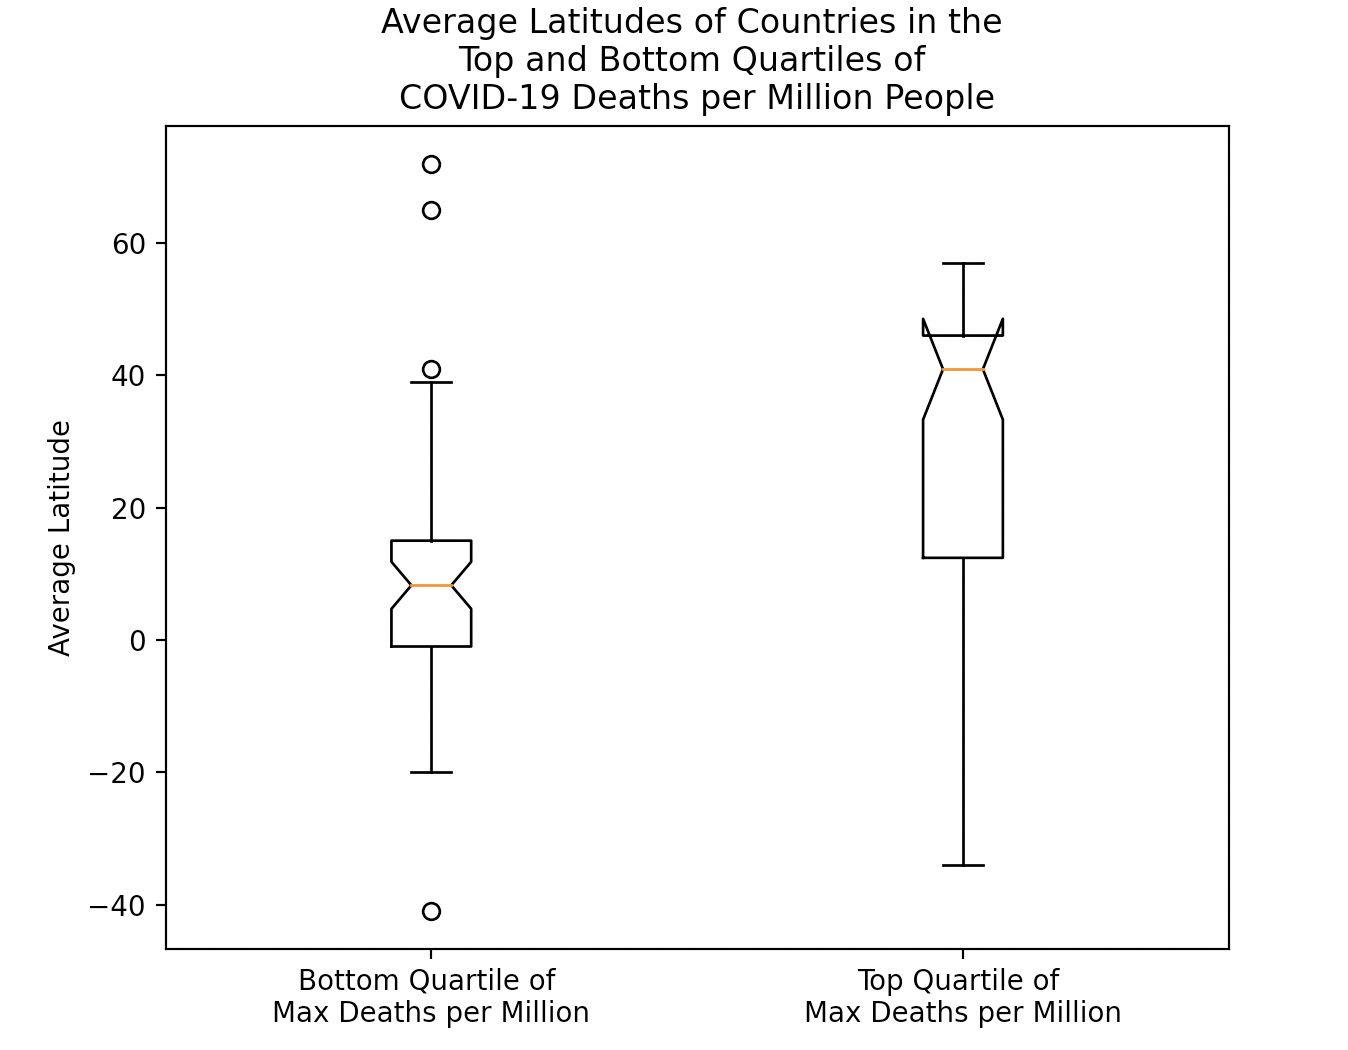
\includegraphics[scale = .33]{boxplot_4.png}
    \]  
\end{enumerate}
    We can see that countries in the lower quartile of deaths are much closer to the equator (latitude 0),
    while countries in the top quartile of deaths are much farther north. This suggests that 
    COVID-19 deaths can be linked to climate. In countries farther north, there is likely a colder climate 
    for much of the year, which may exacerbate COVID symptoms and increase the spread. \\ \\
    Conversely, in warmer climates, COVID doesn't spread as much due to the heat or 
    perhaps an increase in Vitamin D consumption, from more exposure to sunlight has 
    a positive affect on the immune systems ability to fight COVID. More experiments would 
    need to be conducted to make conclusions on these new hypothesis. 
\end{document}